main.tex is the main file, outlining all the section. Please take your lecture note into Ch\ref{Ch2.1}

Change word size \tiny{Hi} \Huge{Hi} \Large{Hi}

Change word color \textcolor{red}{Hi} \textcolor{blue}{Hi}

Italic:\textit{Hi}

Bold:\textbf{Hi}

Put a pic here
\begin{figure}[htb]
\centering
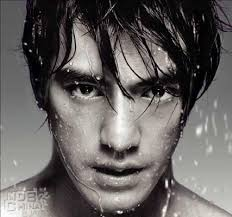
\includegraphics[width=0.5\textwidth]{FIG/mypic.jpg}
\caption{This is me}
\label{mypic}
\end{figure}

Fig.\ref{mypic} is my picture.

We define some commands in dft.tex, before you type a new label, please check it is already exist or not. For example, Dr.\ Da-Cheng Juan is \DC\@. You can add your new command into dft.tex, but also add comment and used in which chapter.

Math inline mode:\\
A polynomial: $x^{3} + 2x^{2} + x$\\
A series: $a_{1}, a_{2}, a_{3}, a_{4}, a_{5}$\\
$x^{2y^{3}}$ $x^{2y_{2}}$ $x^{y}_{1}$ $x_{1}^{y}$\\

Math display mode:\\
\[
\sum_{i=1}^{n}{n^2-3n+4} = f(n)
\]
\begin{equation}
\label{myequation}
\sum_{i=1}^{n}{n^2-3n+4} = f(n)
\end{equation}

